
\title{Report on the ITER Clite Shutdown Doserate Calculations}
\author{
  Andrew Davis \\
  Department of Engineering Physics\\
  College of Engineering \\
  The University of Wisconsin-Madison\\
  Madison, Wisconsin, 53706, \underline{USA}
  \and
  Mohamed Sawan \\
  Department of Engineering Physics\\
  College of Engineering \\
  The University of Wisconsin-Madison\\
  Madison, Wisconsin, 53706, \underline{USA}
  \and
  Elliott Biondo \\
  Department of Engineering Physics\\
  College of Engineering \\
  The University of Wisconsin-Madison\\
  Madison, Wisconsin, 53706, \underline{USA}
  \and
  Patrick Shriwise \\
  Department of Engineering Physics\\
  College of Engineering \\
  The University of Wisconsin-Madison\\
  Madison, Wisconsin, 53706, \underline{USA}
}

\date{\today}

\documentclass[12pt]{article}
\usepackage{graphicx}
\usepackage[a4paper, portrait, margin=0.5in]{geometry}
\usepackage[table]{xcolor}

\begin{document}
\maketitle
\newpage
==\tableofcontents
\newpage
\section{Introduction}
The shutdown doserate in an around the equatorial and upper ports determine the type and duration of maintenance that can be
performed by person access. Thus, minimization of the dose rate is desirable and indeed encouraged by the ALARA principles used
at ITER. It was recently suggested that lining the plasma side of the concrete bioshield with a thin ($\sim$ mm thickness) layer of boron carbide (B$_4$C) would be inexpensive to install and absorb much of the thermal flux which would otherwise lead to neutron
induced activation. Simple scoping calculations suggest that the thermal neutron flux should be depressed significantly and lead
to signficantly lower shutdown photon doserates. The main goal of this report was therefore to examine if the use of the B4C liner
does indeed lead to lower doserates.

\section{The CAD Model}
The CAD model was generated from several source, ITER Clite CAD, IO Diagnostics, previous MCNP analysis which were detailed in \cite{cad_origination}. The model represents several ITER systems in high levels of detail, with all detail retained in the Equatorial Port Interspace (EPI), the  Upper Port Interspace (UPI), and the Lower Port Cryopump.
\subsection{Clite CAD Model}
The overall CAD model in shown in Figure \ref{fig:cad_iter_global}, the broad details of the model can be seen.
\begin{figure}[p]
  \centering
  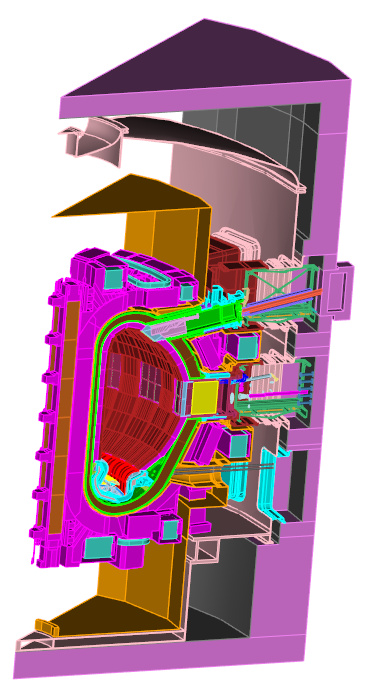
\includegraphics[scale=0.8]{../plots/cad/global.png}
  \caption{Section showing the overall model}
  \label{fig:cad_iter_global}
\end{figure}

\begin{figure}[p]
  \centering
  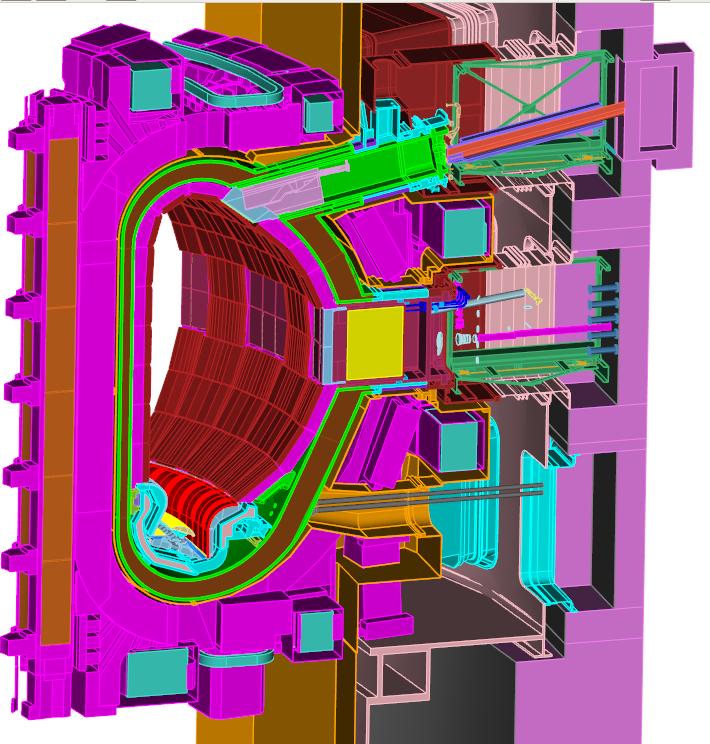
\includegraphics[scale=0.8]{../plots/cad/global_zoom.png}
  \caption{Section showing the overall model}
  \label{fig:cad_iter_global_zoom}
\end{figure}

\subsection{Materials}
All materials in the problem originate from the Clite MCNP model - CLITE\textunderscore V1\textunderscore REV131031\textunderscore MOD, with the exception of the Upper Port Plugs (UPP), the Equatorial Port Plug (EPP), the Cryopump, and the contents of the UPI and EPI. The default cross section set used was FENDL-2.1, with the exception of XX which was expanded into an isoptopic defintion and used the ENDF-VIIR1 evaluation. The EPP material definitions were taken from the Generic Equatorial Port Plug (GEPP) MCNP model \cite{epp_materials}. The UPP material definitions were provided by \cite{bertalot_communication}. The Cryopump materials assignments came from \cite{cryopump_communication}. The full evaluated material definitions can be found in the Appendix.
\subsection{Variance Reduction}
The weight window parameters were generated using the Oak Ridge National Laboratory (ORNL) code ADVANTG, specifically using DAG-ADVANTG, which allows a DAGMC geometry to be read and the geometry and material data handed off to Denovo. The weight windows used
for the problem are shown below in Figure \ref{fig:wwinp}. The weight windows were produced using the Forward Weighted Consistent Adjoint Driven Importance Sampling (FW-CADIS), which attempts to produce a weight window map which tries to get particles everywhere int the model, as opposed to CADIS for example, which attempts to get results to a small number of specific regions.
\begin{figure}[ht!]
  \centering
  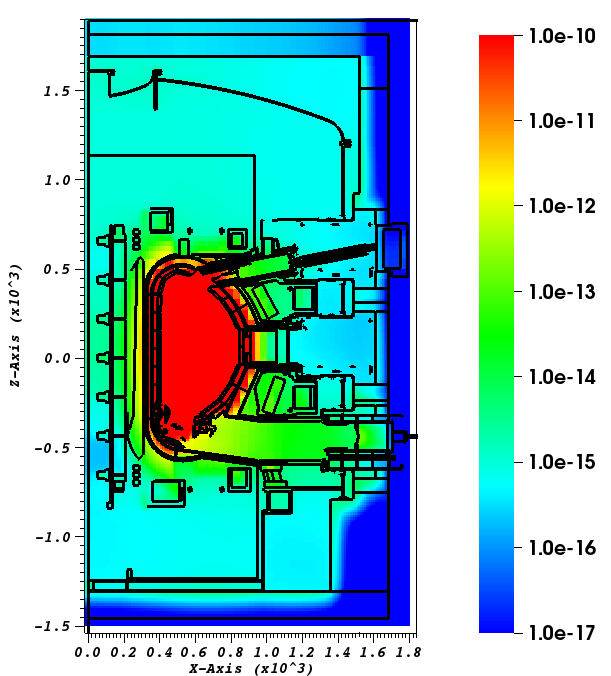
\includegraphics[scale=0.4]{../plots/wwinp/wwinp_y0.png}
  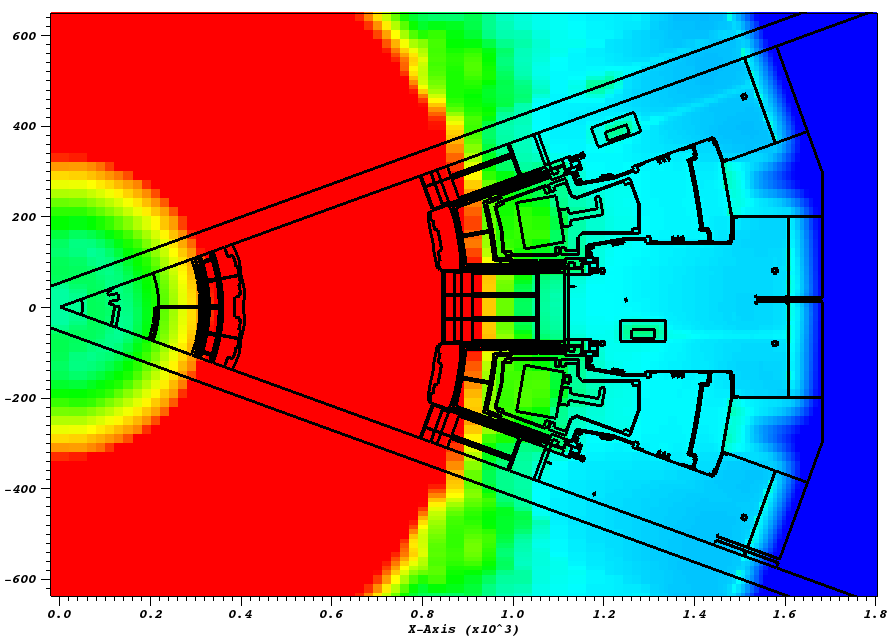
\includegraphics[scale=0.3]{../plots/wwinp/wwinp_z0.png}
  \caption{Slices through the ADVANTG produced weight window through y = 0.0 cm and through z = 0.0 cm}
  \label{fig:wwinp}
\end{figure}
Several artifacts are worthy of note, despite being a deterministic code Denovo has handled the streaming of neutrons along the divertor duct well as shown in left hand image of Figure \ref{fig:wwinp}. The overall span of the weight window is seven orders of magnitude, which is largely proportional to the neutron attenuation from the plasma to the port interspace, previous calculations put the attenuation in the range of 6 to 8 orders of magnitude. There is some evidence of ray effects in the weight window solution in the right hand image of Figure \ref{fig:wwinp} due to the neutron attenuation of some EPI shielding around the diagnostic equipment, but this is small deviation in an otherwise reasonable solution.
\\
\\
It should be noted that ORNL specifically developed the 360$^{\circ}$ rotation feature for DAG-ADVANTG that allows rotationally symmetric bodies, which is the reason for the weight window values beyond the 40$^{\circ}$ sector. 

\section{Neutron Transport Results}
The neutron transport calculations were performed using version 1.0 of DAG-MCNP5 using the source from version 1.60 of MCNP5, from the develop branch with git checkout \texttt{e12e2a3}. The two batches of calculations one for the with B$_4$C case and one without, were submited to the University of Wisconsin's Centre for High Throughput Computer (CHTC) system in batches of 200, with seven meshes used to determine the neutron flux, making a total of 2800 individual MCNP simulations. These results were then combined using PyNE to result in the statistically averaged final results. Intially calculations were batched into groups of $5\times10^7$ particles per batch, however these calculations did not finish in a timely enough manner and were instead reduced to groups of $5\times10^6$ particles per batch. 
\subsection{Including the B4C Liner}
\begin{figure}[ht!]
  \centering
  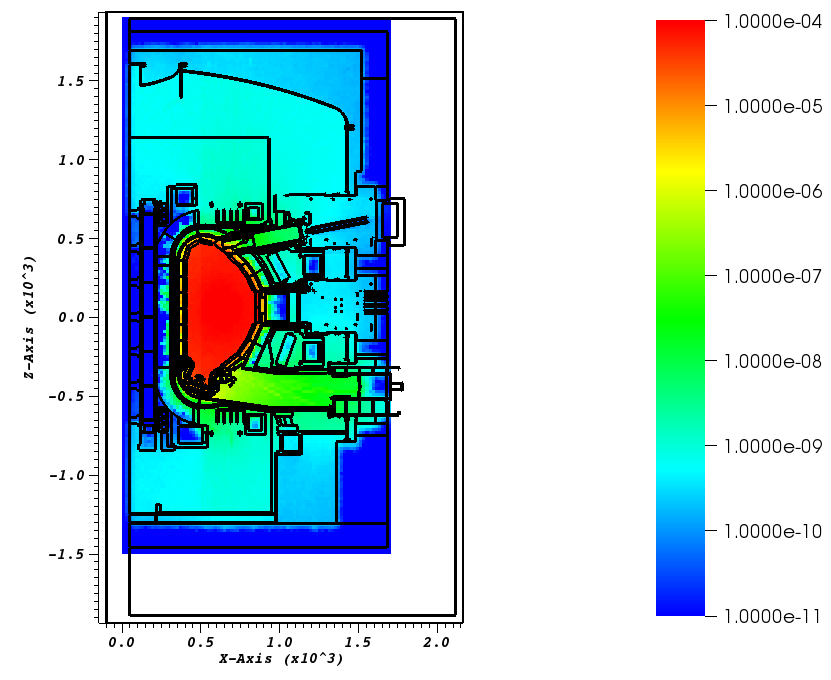
\includegraphics[scale=0.4]{../plots/neutron/b4c/flux_y-17.png}
  \caption{Slices through the total neutron flux (n cm$^{-2}$ src$^{-1}$) y = -17.0 cm and through z = 0.0 cm}
  \label{fig:wwinp}
\end{figure}
\begin{figure}[ht!]
  \centering
  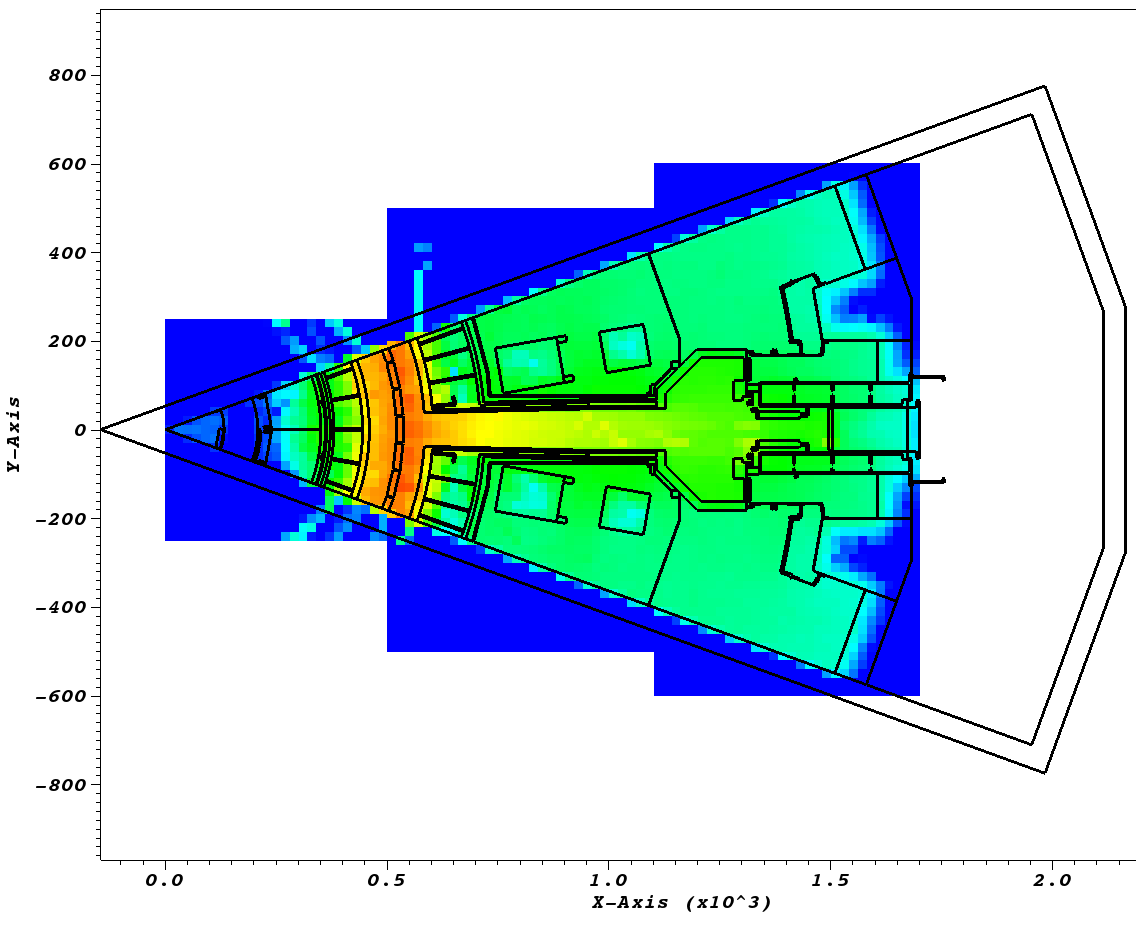
\includegraphics[scale=0.27]{../plots/neutron/b4c/flux_z-500.png}
  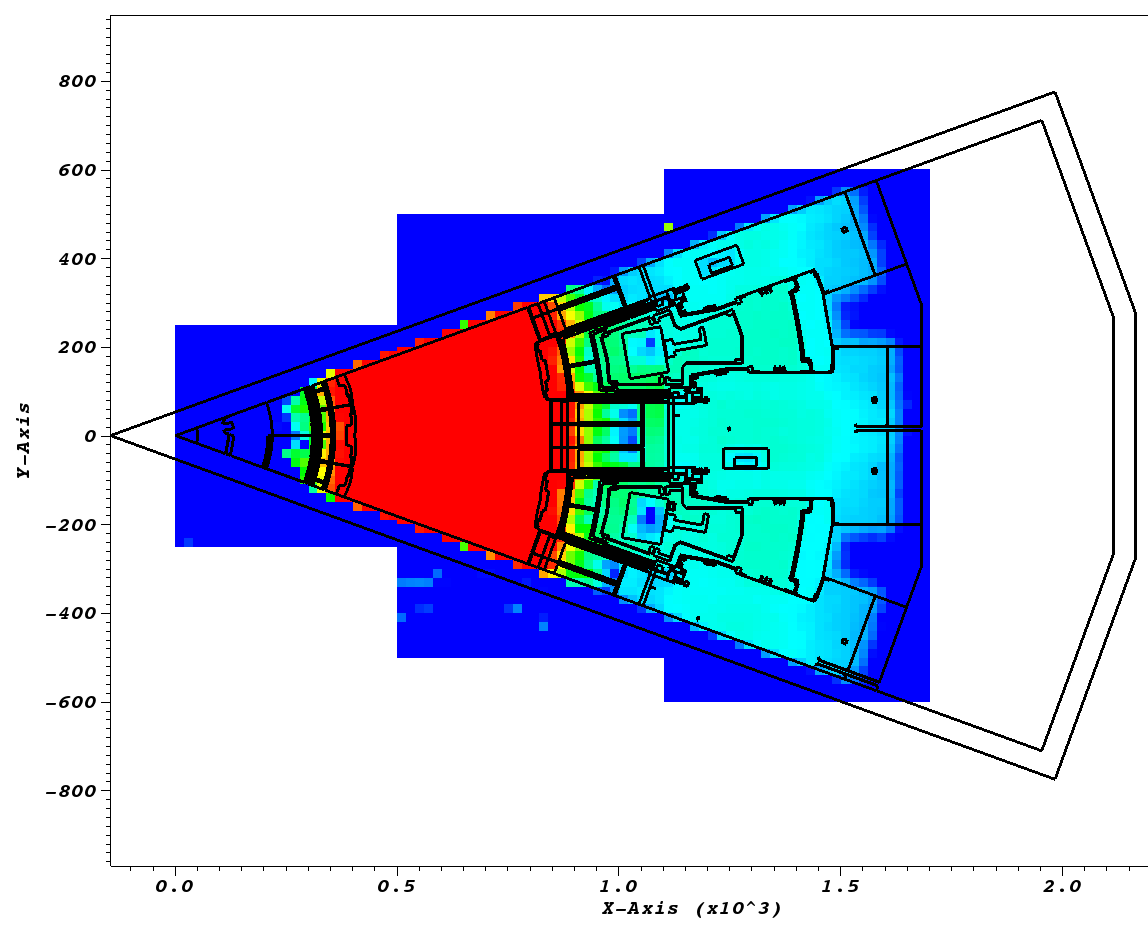
\includegraphics[scale=0.27]{../plots/neutron/b4c/flux_z0.png}       
  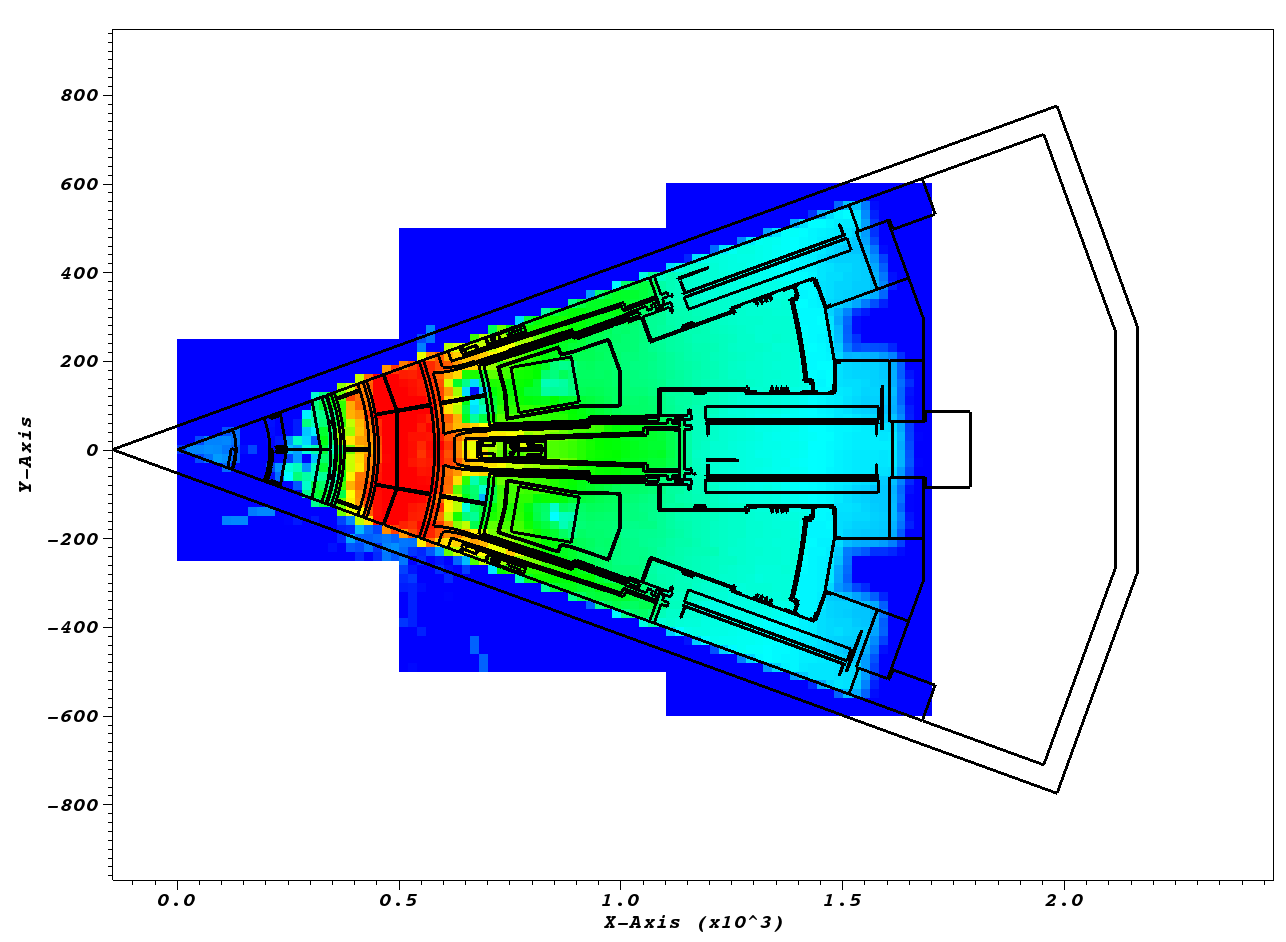
\includegraphics[scale=0.27]{../plots/neutron/b4c/flux_z500.png}
  \caption{Slices through the total neutron flux (n cm$^{-2}$ src$^{-1}$) z = -500.0 cm and through z = 500.0 cm}
  \label{fig:wwinp}
\end{figure}

\subsection{Without the B4C Liner}
\section{Neutron Activation}
The R2S shutdown dose rate calculations were performed using the pyne.r2s methods found PyNE. The setup scripts produce Alara input
and the neutron activation calculations were performed using Alara 2.9.1RC which used the FENDL-3.0/A activation cross sections.
The calculations were broken up into meshes where are of an appropriate size to fit on a machine with 24 Gb of physical RAM. These
Alara calculations are run and then photon sources produced for each of the 3 decay times that were investigated.

\subsection{Irradiation Scenario}

\begin{table}
   \begin{tabular}{| l | c |}
      \hline 
      Irradiation Period & Fractional Strength \\
      \hline
      5 Years & 0.0095 \\
      1 Year  & 0.0127 \\
      1 Year  & 0.0190 \\
      1 Year  & 0.0317 \\
      1 Year  & 0.0380 \\
      1 Year  & 0.0380 \\
      6 Days  & 0.1929 \\
      1 Year  & 0.0380 \\
      \cellcolor{blue!25} 400 Seconds & 1.0000 \\
      \cellcolor{blue!25}1673.6 Seconds & 0.0000 \\
      400 Seconds & 1.0000 \\
      \hline
\end{tabular}
\caption{The table shows the ITER-DRG2 scenario for aggresive pulsing, note the cells in \textcolor{blue!25}{blue} are repeated 249
 times}
\label{tag:irrad_scenario}
\end{table}

\subsection{Including the B4C Liner}
\subsection{Without the B4C Liner}
\section{Shutdown Photon Doserates}
The shutdown photon sources were developed in several seperate meshes and therefore any individual mesh does not represent the
entire problem. Each source is run independently, and the photon dose is recorded on a mesh common to each photon calculation and
then the meshes summed together to create the final result. The final mesh has a uniform size of side 2 cm striding from
x = {0,1500}, y = {-500,500}, z = {-1900,1500} cm.
\subsection{Decay time 1 - 1.$\times$10$^5$ s}
\subsection{Decay time 2 - 1.$\times$10$^6$ s}
\subsection{Decay time 3 - 1.$\times$10$^7$ s}

\section{Conclusions}
\subsection{Neutron Transport}
The final calulcations represent only around 10\% of the overall requested runtime, this is mostly due to calculations not completing with the 3 day allotted runtime on CHTC, the reason being that is seems the requested VR parameters were too extreme resulting in severe oversplitting of particles. This has been noticed to occur in several previous challenging attenuating geometries and has been attributed to so called long histories. The long history problem requires an ultimate solution beyond the scope of this report, but perhaps solutions like that already underway at UW-Madison \& ORNL; GT-CADIS \& MS-CADIS respectively.
\subsection{Shutdown Photon Doserate}
It is clear from Figures XXX that the shutdown photon doserate in the port interspaces is significantly affected by the addition of boron carbide to the plasma side surface of the bioshield. The reason for the this is significantly degraded thermal flux which impacts the inportance of (n,$\gamma$) reactions and also the transport of neutrons back from the bioshield. 

\bibliographystyle{amsplain}
\bibliography{bibliography}

\end{document}
This is never printed
